\subsection{Exogenous IFIT2-FLAG Localisation in the Context of RSV pIBs and IBs} \label{subsec:Exogenous IFIT2-FLAG Localisation in the Context of RSV pIBs and IBs}
\subsubsection{IFIT2-FLAG in a Simplified System of pseudo-IBs} \label{IFIT2-FLAG in a Simplified System of pseudo-IBs}
%Exogenous Human and Bovine IFIT2 in pBs
%i2a vero hi2 + hnhp
Cell Line: VERO \newline
Treatment: hNhP + hIFIT2-FLAG \newline
Detecting magenta: endogenous monkey IFIT2 + exogenous human IFIT2 \newline
Detecting cyan: human pIB \newline

Monkey cells transfected with human RSV N and P, along with human IFIT2-FLAG show concentration within the pIB structures as well as the pIB filamentous network. In this experiment we are detecting both human and monkey IFIT2, however we can see a huge difference in IFIT2 expression between some cells (bottom panel; cells in the periphery of the picture), suggesting that what we are mainly detecting is the overexpressed human IFIT2-FLAG.

\begin{figure}
    \begin{subfigure}{0.5\textwidth}
        \caption{}
        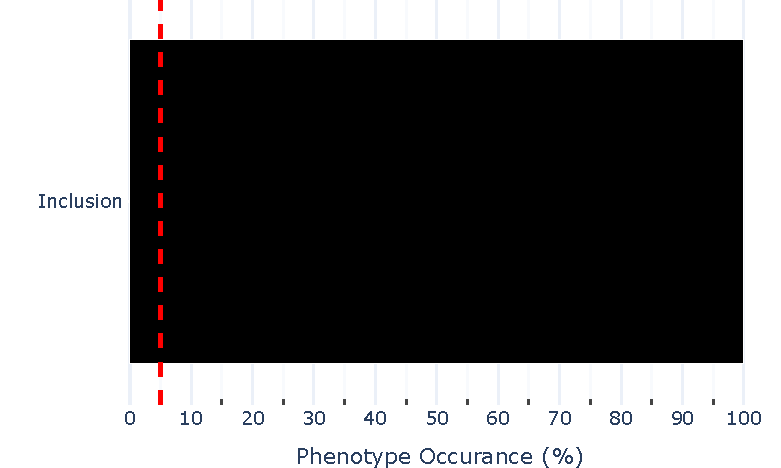
\includegraphics[width=1\linewidth]{10. Chapter 5/Figs/03. IFIT2-FLAG/01. IFIT2A/01. bar_i2a_hnhp.pdf} 
    \end{subfigure}
    \begin{subfigure}{0.5\textwidth}
        \caption{}
        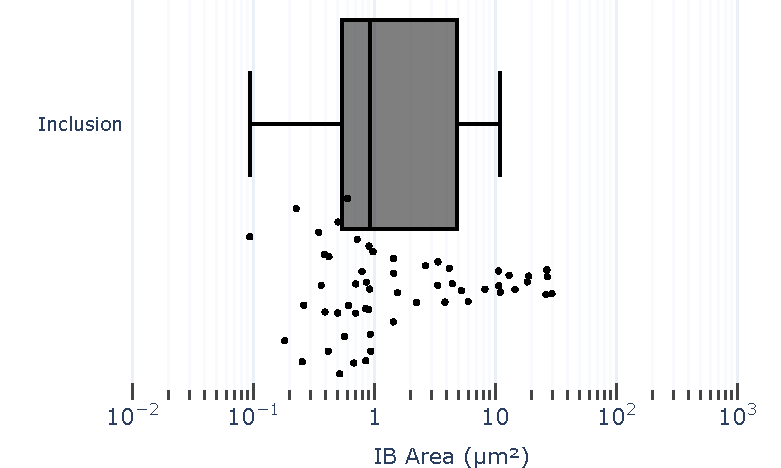
\includegraphics[width=1\linewidth]{10. Chapter 5/Figs/03. IFIT2-FLAG/01. IFIT2A/02. box_i2a_hnhp.pdf}
    \end{subfigure}
    \begin{subfigure}{1\textwidth}
        \centering
        \caption{}
        \includegraphics[width=1\linewidth]{10. Chapter 5/Figs/03. IFIT2-FLAG/01. IFIT2A/03. i2a-hi2f-hnhp.pdf}
    \end{subfigure}
    \caption[i2a vero hi2 + hnhp]{\textbf{i2a vero hi2 + hnhp.} Nascent bovine IFIT1 in the context of bRSV infection has been observed to localise with the respect of IB in three distinct spaces. We observed it either concentrated inside the central point of the IB structure, while having reduced signal on the inner IB edge, compared to the cytoplasm (top and bottom panels), being excluded from the IB structure (3rd panel), or colocalising on the inner edge of the IB structure while having reduced signal in the middle of the structure compared to cytoplasm, or the edge staining (2nd panel).}
    \label{fig:i2a vero hi2 + hnhp}
\end{figure}

%Exogenous Human and Bovine IFIT2 in pBs
%i2b vero hi2 + hnhp
Cell Line: VERO \newline
Treatment: hNhP + hIFIT2-FLAG \newline
Detecting magenta: endogenous monkey IFIT2 + exogenous human IFIT2 \newline
Detecting cyan: human pIB \newline

Monkey cells transfected with human RSV N and P, along with human IFIT2-FLAG show concentration within the pIB structures but show exclusion from the pIB filamentous network (or partial colocalsiation?). This suggest that the IFIT2B antibody can indeed detect IFIT2 but the overexpressed IFIT2 observed between the inclusion and the one interacting with the filamentous network is somehow different (epitope masking?).

\begin{figure}
    \begin{subfigure}{0.5\textwidth}
        \caption{}
        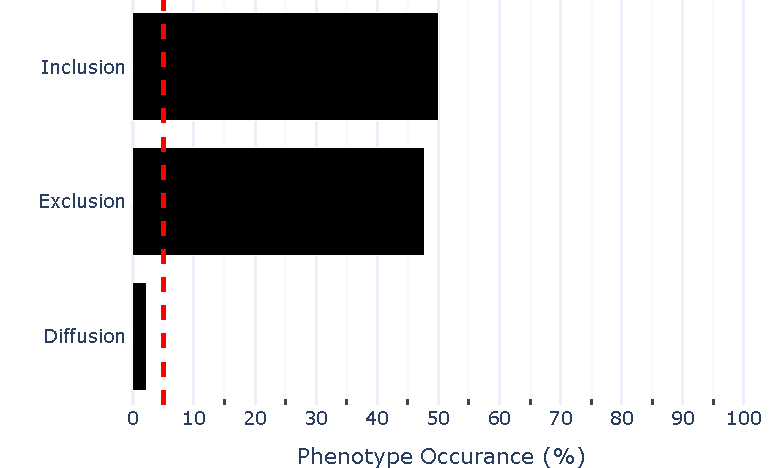
\includegraphics[width=1\linewidth]{10. Chapter 5/Figs/03. IFIT2-FLAG/02. IFIT2B/01. bar_i2b_hnhp.pdf} 
    \end{subfigure}
    \begin{subfigure}{0.5\textwidth}
        \caption{}
        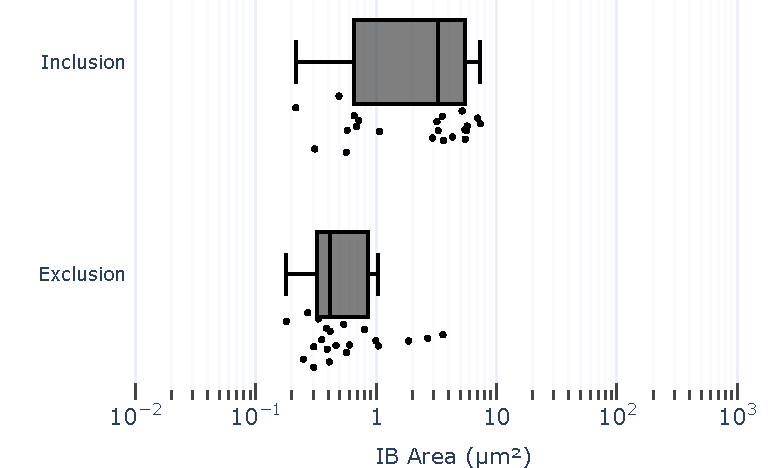
\includegraphics[width=1\linewidth]{10. Chapter 5/Figs/03. IFIT2-FLAG/02. IFIT2B/02. box_i2a_hnhp.pdf}
    \end{subfigure}
    \begin{subfigure}{1\textwidth}
        \centering
        \caption{}
        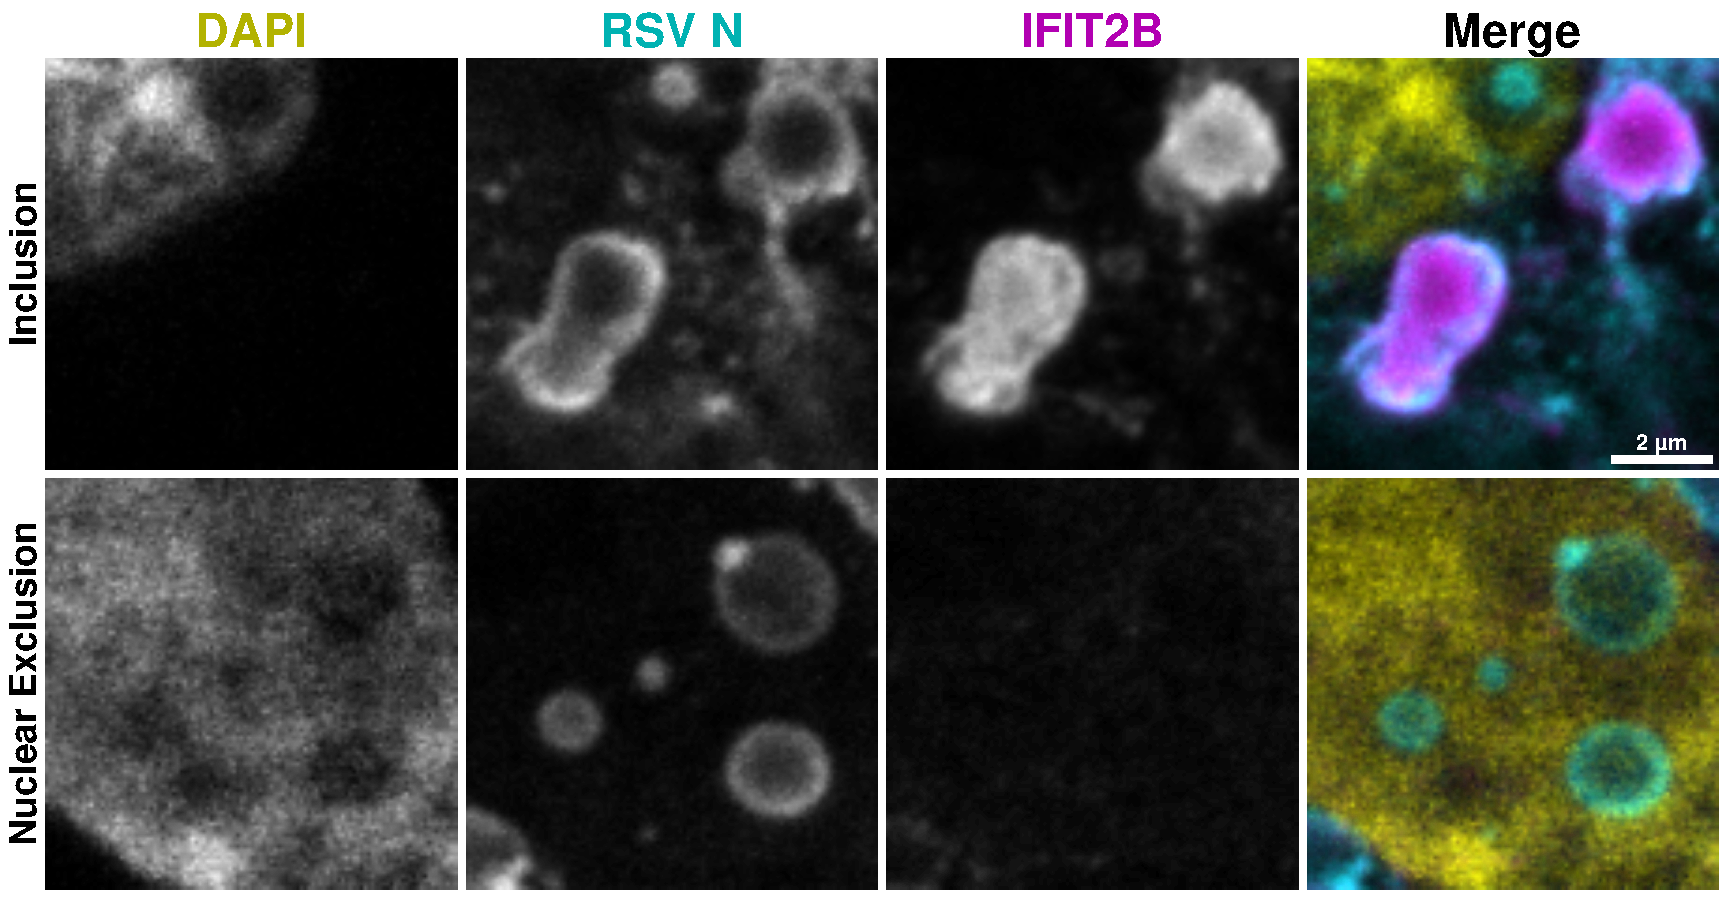
\includegraphics[width=1\linewidth]{10. Chapter 5/Figs/03. IFIT2-FLAG/02. IFIT2B/03. i2b-hi2f-hnhp.pdf}
    \end{subfigure}
    \caption[i2b vero hi2 + hnhp]{\textbf{i2b vero hi2 + hnhp.} Nascent bovine IFIT1 in the context of bRSV infection has been observed to localise with the respect of IB in three distinct spaces. We observed it either concentrated inside the central point of the IB structure, while having reduced signal on the inner IB edge, compared to the cytoplasm (top and bottom panels), being excluded from the IB structure (3rd panel), or colocalising on the inner edge of the IB structure while having reduced signal in the middle of the structure compared to cytoplasm, or the edge staining (2nd panel).}
    \label{fig:i2b vero hi2 + hnhp}
\end{figure}

%hi2f hnhp
Cell Line: VERO \newline
Treatment: hNhP + hIFIT2-FLAG \newline
Detecting magenta: exogenous human IFIT2 \newline
Detecting cyan: human pIB \newline

Exogenously expressed human IFIT2 colocalises with the pIB associated filamentous net (top panel). It also forms inclusion inside the human pIB structures. This data is consistent with what we observed with IFIT2A antibody. IFIT2 also seems to occasionally form aggregates/spots (highlighted by arrows). These could be functional or just aggregates caused by overexpression, we do not know.

\begin{figure}
    \begin{subfigure}{0.5\textwidth}
        \caption{}
        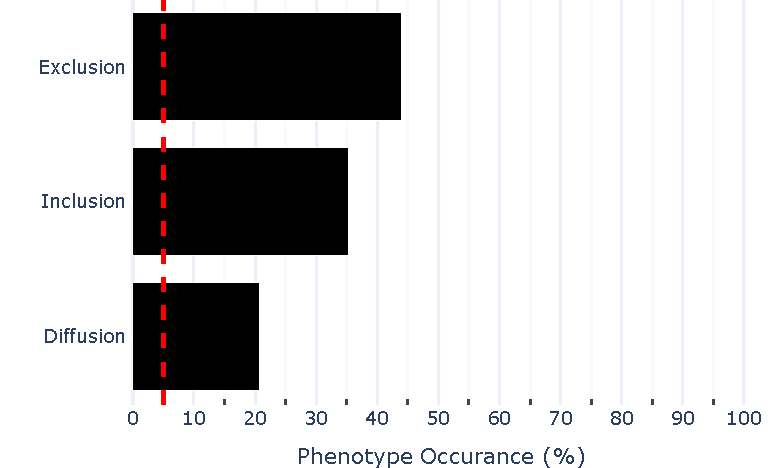
\includegraphics[width=1\linewidth]{10. Chapter 5/Figs/03. IFIT2-FLAG/03. IFIT2F/01. pIB/01. bar_hi2f_hnhp.pdf} 
    \end{subfigure}
    \begin{subfigure}{0.5\textwidth}
        \caption{}
        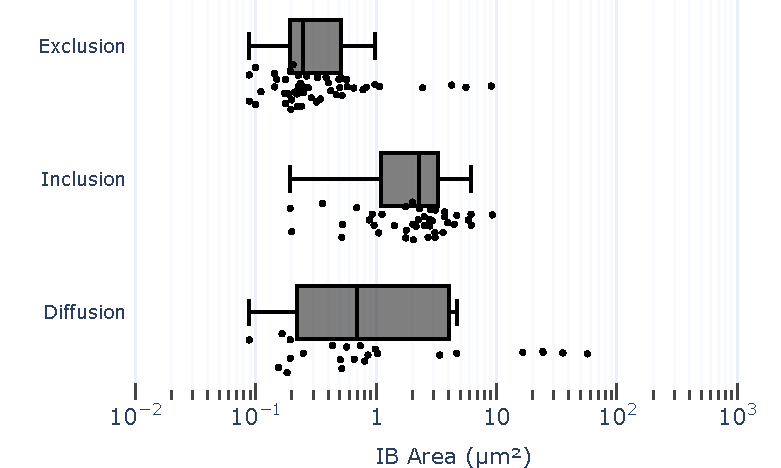
\includegraphics[width=1\linewidth]{10. Chapter 5/Figs/03. IFIT2-FLAG/03. IFIT2F/01. pIB/02. box_hi2f_hnhp.pdf}
    \end{subfigure}
    \begin{subfigure}{1\textwidth}
        \centering
        \caption{}
        \includegraphics[width=1\linewidth]{10. Chapter 5/Figs/03. IFIT2-FLAG/03. IFIT2F/01. pIB/03. hi2f-hnhp.pdf}
    \end{subfigure}
    \caption[hi2f hnhp]{\textbf{hi2f hnhp.} Nascent bovine IFIT1 in the context of bRSV infection has been observed to localise with the respect of IB in three distinct spaces. We observed it either concentrated inside the central point of the IB structure, while having reduced signal on the inner IB edge, compared to the cytoplasm (top and bottom panels), being excluded from the IB structure (3rd panel), or colocalising on the inner edge of the IB structure while having reduced signal in the middle of the structure compared to cytoplasm, or the edge staining (2nd panel).}
    \label{fig:hi2f hnhp}
\end{figure}

%bi2f hnhp
Cell Line: VERO hSLAM \newline
Treatment: hNhP + bIFIT2-FLAG \newline
Detecting magenta: exogenous bovine IFIT2 \newline
Detecting cyan: human pIB \newline

Exogenous bovine IFIT2 colocalises with the edge of human pIB structures. This is unusual as human IFIT2 data suggest inclusions with regards to pIBs.

\begin{figure}
    \begin{subfigure}{0.5\textwidth}
        \caption{}
        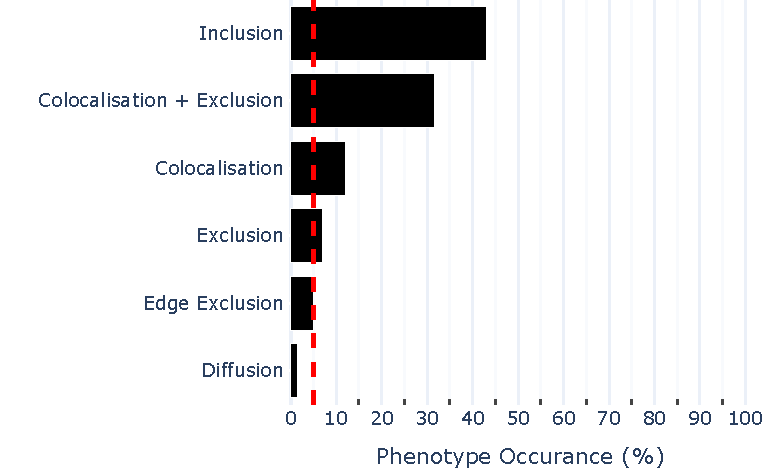
\includegraphics[width=1\linewidth]{10. Chapter 5/Figs/03. IFIT2-FLAG/03. IFIT2F/01. pIB/04. bar_bi2f_hnhp.pdf} 
    \end{subfigure}
    \begin{subfigure}{0.5\textwidth}
        \caption{}
        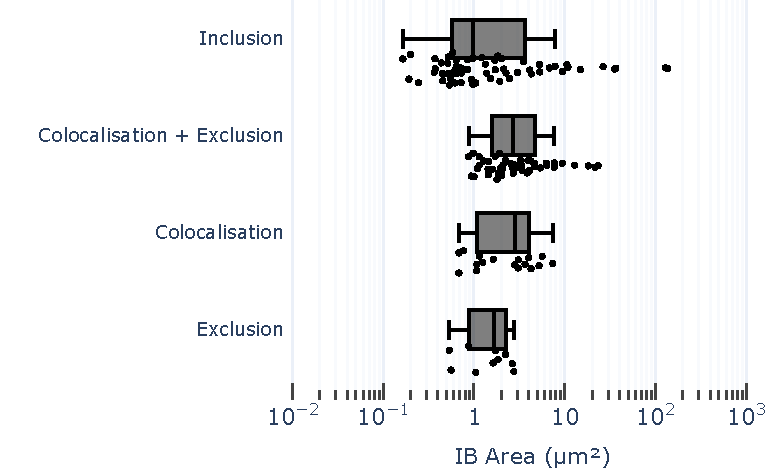
\includegraphics[width=1\linewidth]{10. Chapter 5/Figs/03. IFIT2-FLAG/03. IFIT2F/01. pIB/05. box_bi2f_hnhp.pdf}
    \end{subfigure}
    \caption[bi2f hnhp plots]{\textbf{bi2f hnhp plots.} Nascent bovine IFIT1 in the context of bRSV infection has been observed to localise with the respect of IB in three distinct spaces. We observed it either concentrated inside the central point of the IB structure, while having reduced signal on the inner IB edge, compared to the cytoplasm (top and bottom panels), being excluded from the IB structure (3rd panel), or colocalising on the inner edge of the IB structure while having reduced signal in the middle of the structure compared to cytoplasm, or the edge staining (2nd panel).}
    \label{fig:bi2f hnhp plots}
\end{figure}

\begin{figure}
    \centering
    \includegraphics[width=1\linewidth]{10. Chapter 5/Figs/03. IFIT2-FLAG/03. IFIT2F/01. pIB/06. bi2f-hnhp.pdf}
    \caption[bi2f hnhp]{\textbf{bi2f hnhp.} Nascent bovine IFIT1 in the context of bRSV infection has been observed to localise with the respect of IB in three distinct spaces. We observed it either concentrated inside the central point of the IB structure, while having reduced signal on the inner IB edge, compared to the cytoplasm (top and bottom panels), being excluded from the IB structure (3rd panel), or colocalising on the inner edge of the IB structure while having reduced signal in the middle of the structure compared to cytoplasm, or the edge staining (2nd panel).}
    \label{fig:bi2f hnhp}
\end{figure}

\begin{figure}
    \begin{subfigure}{0.5\textwidth}
        \caption{}
        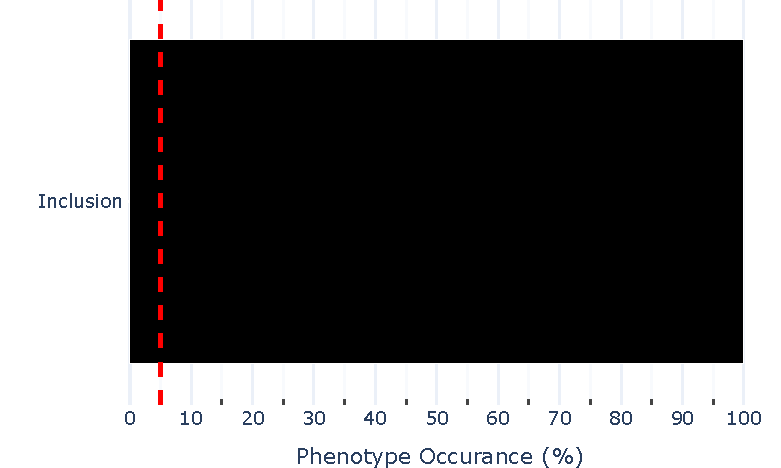
\includegraphics[width=1\linewidth]{10. Chapter 5/Figs/03. IFIT2-FLAG/03. IFIT2F/01. pIB/07. bar_bi2f_bnbp.pdf} 
    \end{subfigure}
    \begin{subfigure}{0.5\textwidth}
        \caption{}
        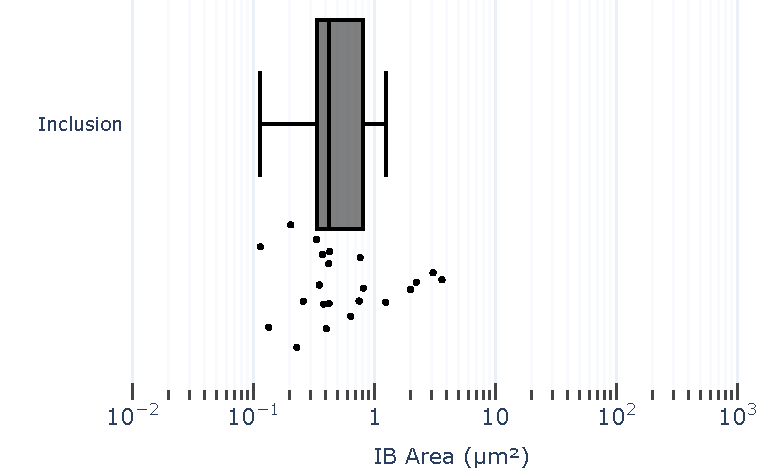
\includegraphics[width=1\linewidth]{10. Chapter 5/Figs/03. IFIT2-FLAG/03. IFIT2F/01. pIB/08. box_bi2f_bnbp.pdf}
    \end{subfigure}
    \begin{subfigure}{1\textwidth}
        \centering
        \caption{}
        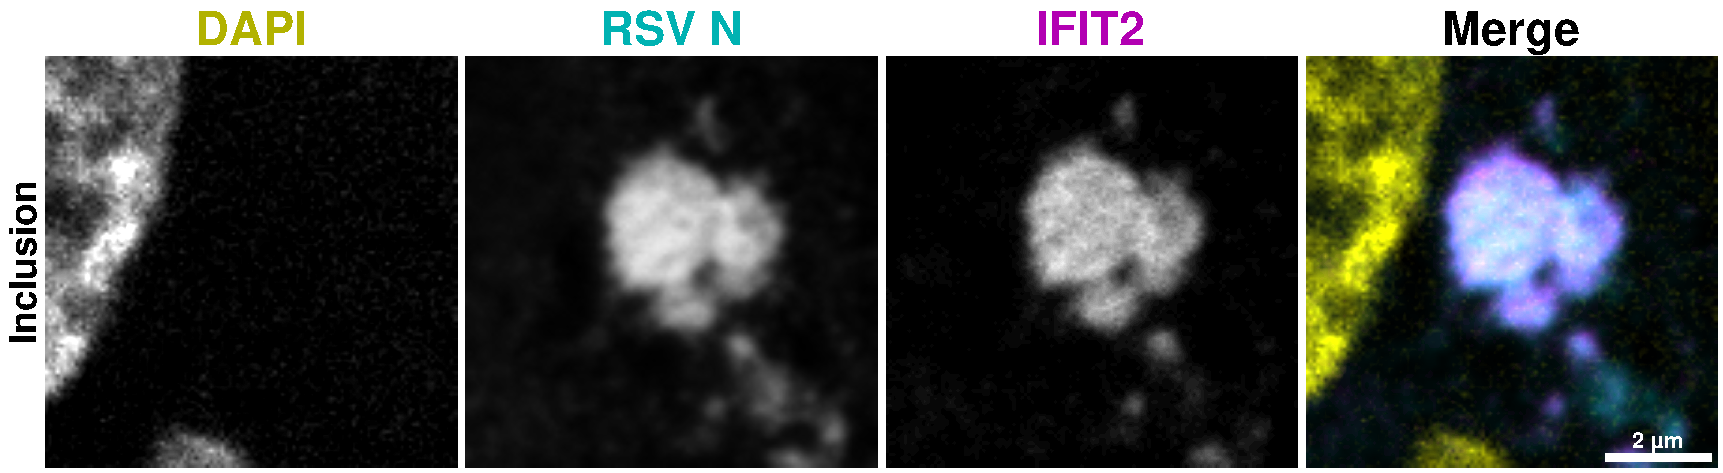
\includegraphics[width=1\linewidth]{10. Chapter 5/Figs/03. IFIT2-FLAG/03. IFIT2F/01. pIB/09. bi2f-bnbp.pdf}
    \end{subfigure}
    \caption[bi2f bnbp]{\textbf{bi2f bnbp.} Nascent bovine IFIT1 in the context of bRSV infection has been observed to localise with the respect of IB in three distinct spaces. We observed it either concentrated inside the central point of the IB structure, while having reduced signal on the inner IB edge, compared to the cytoplasm (top and bottom panels), being excluded from the IB structure (3rd panel), or colocalising on the inner edge of the IB structure while having reduced signal in the middle of the structure compared to cytoplasm, or the edge staining (2nd panel).}
    \label{fig:bi2f bnbp}
\end{figure}

\subsubsection{Exogenous IFIT2-FLAG During RSV Infection} \label{Exogenous IFIT2-FLAG During RSV Infection}
%hi2f hrsv
Cell Line: VERO hSLAM \newline
Treatment: hRSV + hIFIT2-FLAG \newline
Detecting magenta: exogenous human IFIT2 \newline
Detecting cyan: human IB \newline

Overexpressed human IFIT2 during hRSV infection shows several phenotypes (in this experiment). We see IFIT2 being excluded from the IB interior while being concentrated to the IB ring (top panel); IFIT2 forming concentrated inclusion inside the IB structure (2nd panel); IFIT2 being excluded from the IB interior but colocalising to the IB ring and forming spots inside of the IB (3rd panel); and IFIT2 being diffused evenly through the cytoplasm and the IB structure (last panel). The different phenotypes suggest that IBs are dynamic structures, and the localisation depends on factors we do not comprehend yet. 

\begin{figure}
    \begin{subfigure}{0.5\textwidth}
        \caption{}
        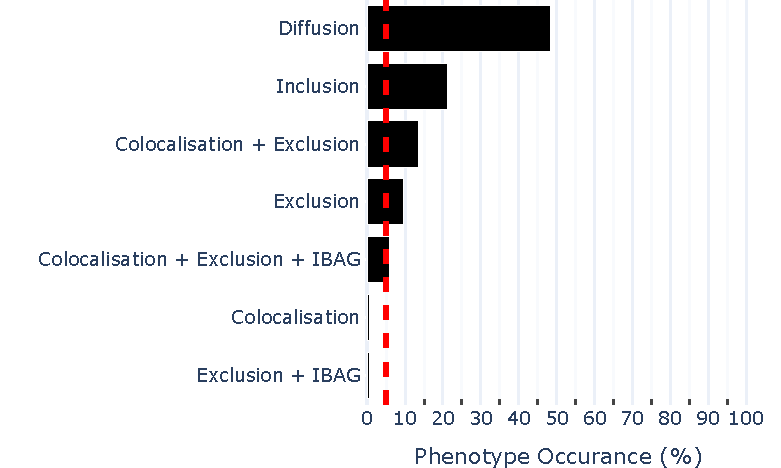
\includegraphics[width=1\linewidth]{10. Chapter 5/Figs/03. IFIT2-FLAG/03. IFIT2F/02. Infection Transfection/01. bar_hi2f_hrsv.pdf} 
    \end{subfigure}
    \begin{subfigure}{0.5\textwidth}
        \caption{}
        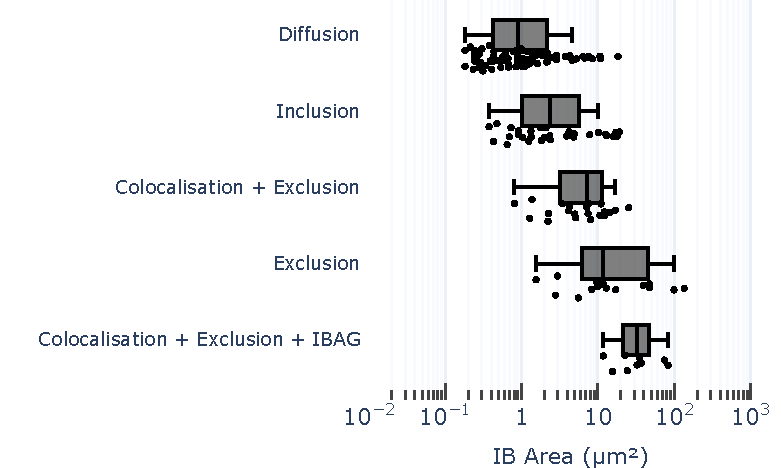
\includegraphics[width=1\linewidth]{10. Chapter 5/Figs/03. IFIT2-FLAG/03. IFIT2F/02. Infection Transfection/02. box_hi2f_hrsv.pdf}
    \end{subfigure}
    \caption[hi2f hrsv plots]{\textbf{hi2f hrsv plots.} Nascent bovine IFIT1 in the context of bRSV infection has been observed to localise with the respect of IB in three distinct spaces. We observed it either concentrated inside the central point of the IB structure, while having reduced signal on the inner IB edge, compared to the cytoplasm (top and bottom panels), being excluded from the IB structure (3rd panel), or colocalising on the inner edge of the IB structure while having reduced signal in the middle of the structure compared to cytoplasm, or the edge staining (2nd panel).}
    \label{fig:hi2f hrsv plots}
\end{figure}

\begin{figure}
    \centering
    \includegraphics[width=1\linewidth]{10. Chapter 5/Figs/03. IFIT2-FLAG/03. IFIT2F/02. Infection Transfection/03. hi2f-hrsv.pdf}
    \caption[hi2f hrsv]{\textbf{hi2f hrsv.} Nascent bovine IFIT1 in the context of bRSV infection has been observed to localise with the respect of IB in three distinct spaces. We observed it either concentrated inside the central point of the IB structure, while having reduced signal on the inner IB edge, compared to the cytoplasm (top and bottom panels), being excluded from the IB structure (3rd panel), or colocalising on the inner edge of the IB structure while having reduced signal in the middle of the structure compared to cytoplasm, or the edge staining (2nd panel).}
    \label{fig:hi2f hrsv}
\end{figure}

%bi2f hrsv
Cell Line: VERO \newline
Treatment: hRSV + bIFIT2-FLAG \newline
Detecting magenta: exogenous bovine IFIT2 \newline
Detecting cyan: human IB \newline

In the follow up experiment, exogenous bovine IFIT2 in the context of human RSV infection shows the same two phenotypes. It is either excluded from the IBs (middle panel) or colocalises with the ring structure of the IBs (top and bottom panel; highlighted with arrows).

\begin{figure}
    \begin{subfigure}{0.5\textwidth}
        \caption{}
        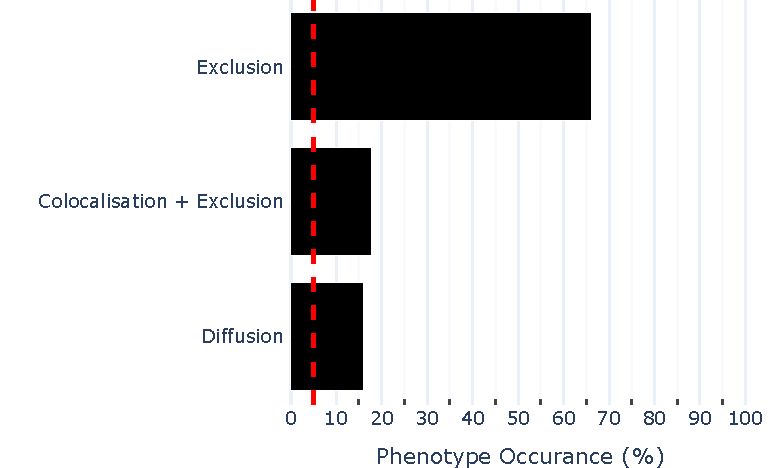
\includegraphics[width=1\linewidth]{10. Chapter 5/Figs/03. IFIT2-FLAG/03. IFIT2F/02. Infection Transfection/04. bar_bi2f_hrsv.pdf} 
    \end{subfigure}
    \begin{subfigure}{0.5\textwidth}
        \caption{}
        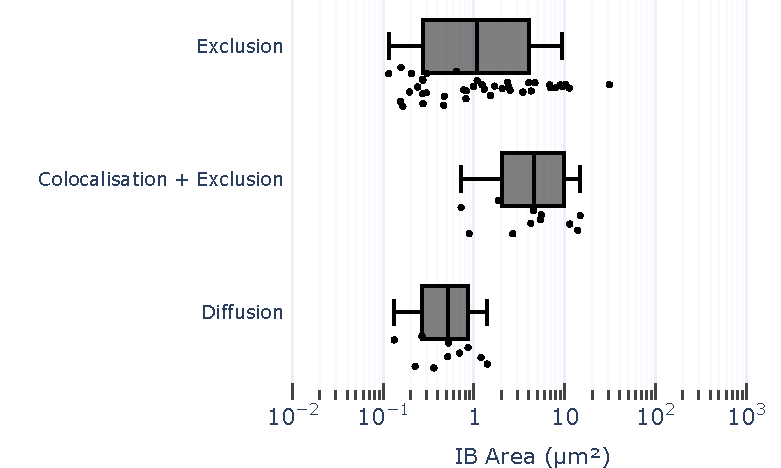
\includegraphics[width=1\linewidth]{10. Chapter 5/Figs/03. IFIT2-FLAG/03. IFIT2F/02. Infection Transfection/05. box_bi2f_hrsv.pdf}
    \end{subfigure}
    \begin{subfigure}{1\textwidth}
        \centering
        \caption{}
        \includegraphics[width=1\linewidth]{10. Chapter 5/Figs/03. IFIT2-FLAG/03. IFIT2F/02. Infection Transfection/06. bi2f-hrsv.pdf}
    \end{subfigure}
    \caption[bi2f hrsv]{\textbf{bi2f hrsv.} Nascent bovine IFIT1 in the context of bRSV infection has been observed to localise with the respect of IB in three distinct spaces. We observed it either concentrated inside the central point of the IB structure, while having reduced signal on the inner IB edge, compared to the cytoplasm (top and bottom panels), being excluded from the IB structure (3rd panel), or colocalising on the inner edge of the IB structure while having reduced signal in the middle of the structure compared to cytoplasm, or the edge staining (2nd panel).}
    \label{fig:bi2f hrsv}
\end{figure}

%bi2f brsv
Cell Line: VERO \newline
Treatment: bRSV + bIFIT2-FLAG \newline
Detecting magenta: exogenous bovine IFIT2 \newline
Detecting cyan: bovine IB \newline

Exogenous bovine IFIT2 during bovine RSV infection seems to be excluded from the inclusion bodies, although the data is not great and the IFIT2 is aggregated in both cells shown.

\begin{figure}
    \begin{subfigure}{0.5\textwidth}
        \caption{}
        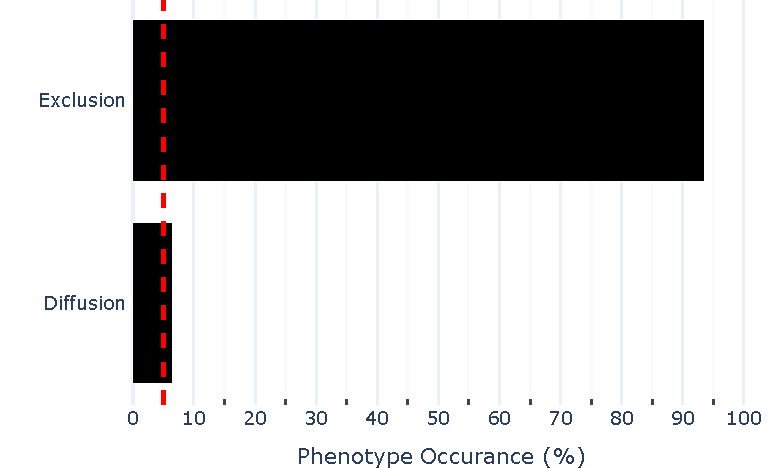
\includegraphics[width=1\linewidth]{10. Chapter 5/Figs/03. IFIT2-FLAG/03. IFIT2F/02. Infection Transfection/07. bar_bi2f_brsv.pdf} 
    \end{subfigure}
    \begin{subfigure}{0.5\textwidth}
        \caption{}
        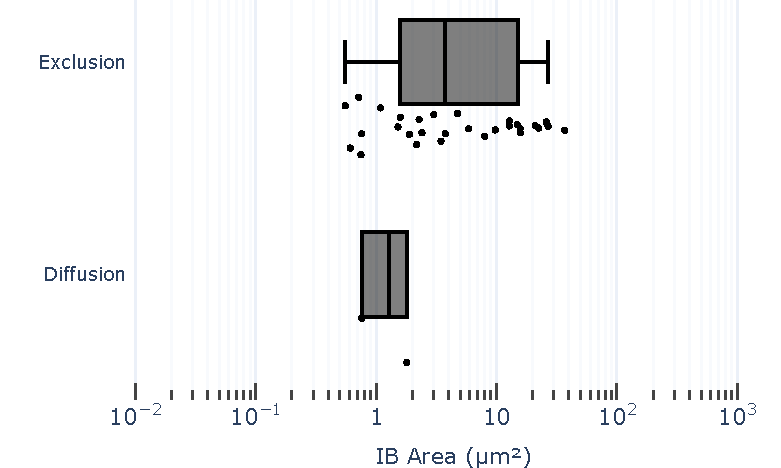
\includegraphics[width=1\linewidth]{10. Chapter 5/Figs/03. IFIT2-FLAG/03. IFIT2F/02. Infection Transfection/08. box_bi2f_brsv.pdf}
    \end{subfigure}
    \begin{subfigure}{1\textwidth}
        \centering
        \caption{}
        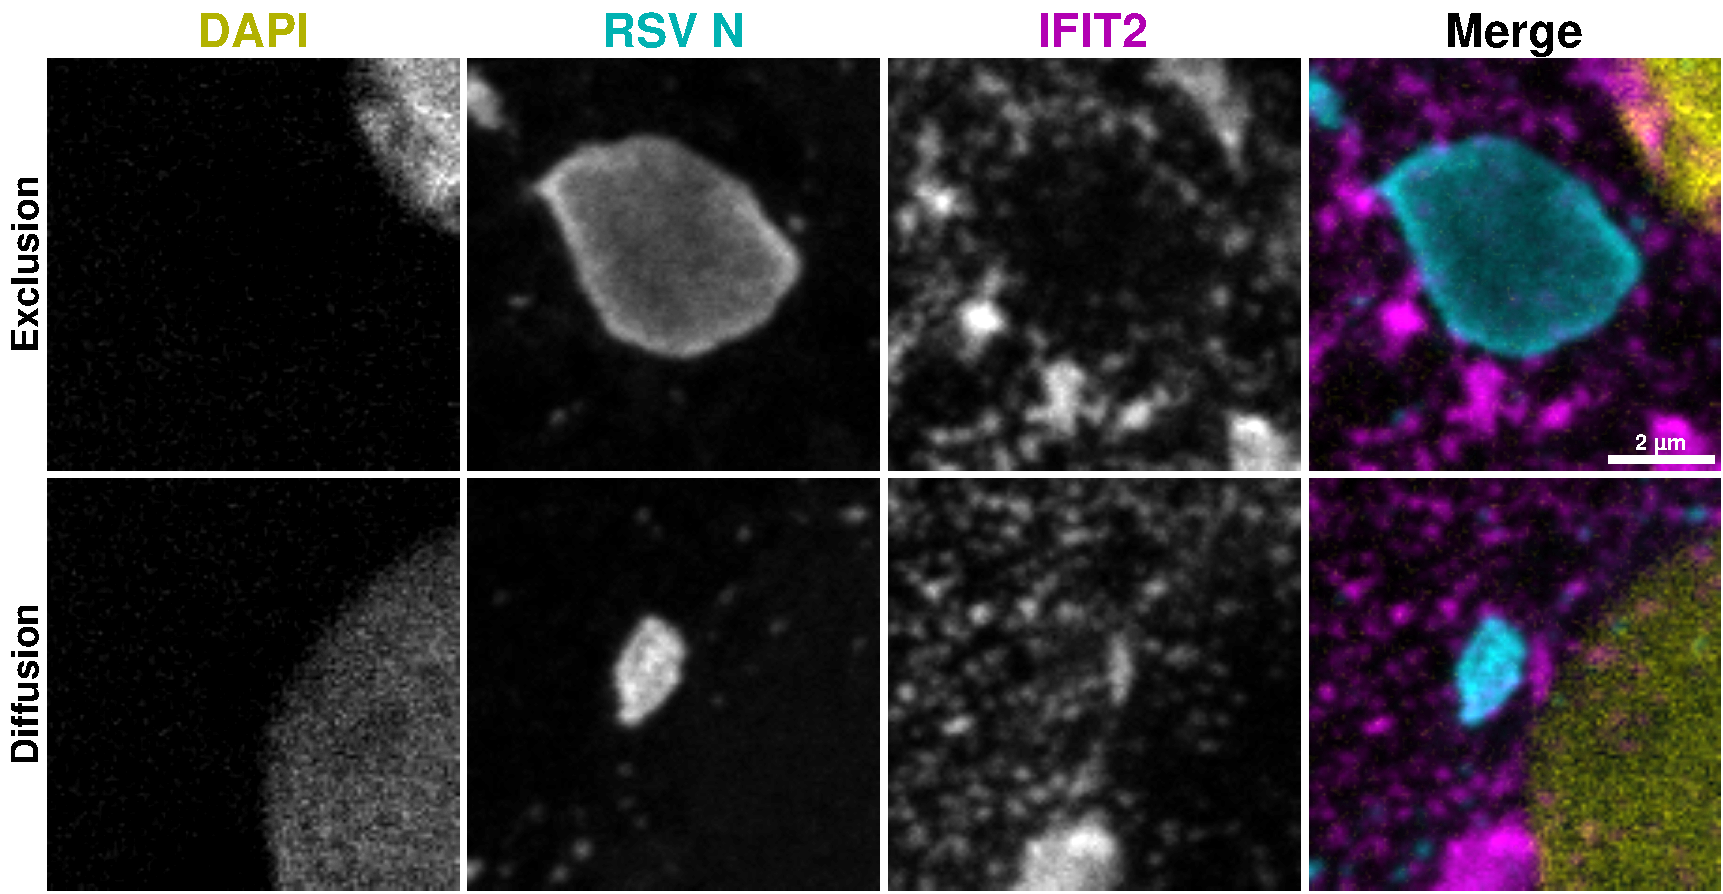
\includegraphics[width=1\linewidth]{10. Chapter 5/Figs/03. IFIT2-FLAG/03. IFIT2F/02. Infection Transfection/09. bi2f-brsv.pdf}
    \end{subfigure}
    \caption[bi2f brsv]{\textbf{bi2f brsv.} Nascent bovine IFIT1 in the context of bRSV infection has been observed to localise with the respect of IB in three distinct spaces. We observed it either concentrated inside the central point of the IB structure, while having reduced signal on the inner IB edge, compared to the cytoplasm (top and bottom panels), being excluded from the IB structure (3rd panel), or colocalising on the inner edge of the IB structure while having reduced signal in the middle of the structure compared to cytoplasm, or the edge staining (2nd panel).}
    \label{fig:bi2f brsv}
\end{figure}

\subsubsection{Summary} \label{Summary-i2-flag}
Overexpressing human IFIT2-FLAG does not seem to be detrimental to the cells. Exogenous human IFIT2 seems to form inclusions inside human pIB structures. It also colocalises with the pIB associated filamentous network. This data is consistent with IFIT2A antibody staining. IFIT2B staining showed inclusion inside pIB but failed to show the colocalization with the filamentous network. Exogenous bovine IFIT2 colocalises to the edge of human pIBs, which is in contrast to what we see with endogenous and exogenous human IFIT2 and its interaction with human pIBs. Exogenous human IFIT2 during human RSV infection showed different phenotypes in 2 different experiments. In the first experiment we observed it to: form inclusions inside the IB structure; be excluded from IB but colocalise to the IB ring; be excluded from the IB but colocalise to the ring and have spots inside the IB structure; or to be diffused through cytoplasm and IB equally. In the second experiment we observed it to be either completely excluded from the IBs or to colocalise with them. Exogenous bovine IFIT2 during human RSV infection was either completely excluded from the IB or was colocalised to the ring of the structure. This was consistently seen in both experiments conducted. Exogenous bovine IFIT2 during bovine RSV infection seems to be excluded from the IBs.